\documentclass[11pt,paper=letter]{scrartcl}
\usepackage[wide]{cjquines}

\begin{asydef}
void vec(pair s, pair v, string l, pair d=0) {
  if (d == 0) {
    d = v-s;
  }
  draw(s--v, arrow=EndArrow(size=5));
  label(l, v, dir(d));
}
\end{asydef}

\begin{document}

\title{Convex combinations}
\subtitle{Tiny Explanations 1}
\author{Carl Joshua Quines}
\date{April 30, 2020}

\maketitle

A \textit{convex combination} of vectors is a linear combination, where all the scalars are non-negative and sum to $1$. In other words, if your vectors were $\vec{v_1}, \vec{v_2}, \ldots, \vec{v_n}$, then a convex combination would be of the form \[
  a_1\vec{v_1} + a_2\vec{v_2} + \cdots + a_n\vec{v_n}
\]
where $a_1, a_2, \ldots, a_n \ge 0$, and $a_1 + a_2 + \cdots + a_n = 1$. These have some nice geometric properties.

\section{Two vectors}

We know what it means to add two vectors, say, $\vec{u} + \vec{v}$. You draw $\vec{u}$, then you draw $\vec{v}$ starting from the tip of $\vec{u}$. Similarly, the interpretation of $\vec{v} - \vec{u}$ is a vector going from the tip of $\vec{u}$ to the tip of $\vec{v}$.
\begin{center}
\begin{asy}
size(9cm);
pair O = (0, 0);
pair U = (-1, 0.75);
pair V = (2, 0.5);

vec(O, U, "$\vec{u}$");
vec(O, V, "$\vec{v}$");
vec(U, U+V, "");
vec(V, U+V, "");
label("$\vec{u} + \vec{v}$", (U+V), N);

pair t = (4, 0);
vec(O+t, U+t, "$\vec{u}$");
vec(O+t, V+t, "$\vec{v}$");
vec(U+t, V+t, "");
label("$\vec{v} - \vec{u}$", (U+V)/2+t, N);
\end{asy}
\end{center}
We can similarly define what $\frac{1}{2}\vec{u} + \frac{1}{2}\vec{v}$ would be. We add half of $\vec{u}$ to half of $\vec{v}$.
\begin{center}
\begin{asy}
size(5cm);
pair O = (0, 0);
pair U = (-1, 0.75);
pair V = (2, 0.5);

vec(O, U, "$\vec{u}$");
vec(O, U/2, "$\frac{1}{2}\vec{u}$", SW);
vec(O, V, "$\vec{v}$");
vec(O, V/2, "$\frac{1}{2}\vec{v}$", SE);
vec(U/2, U/2+V/2, "");
vec(V/2, U/2+V/2, "");
label("$\frac{1}{2}\vec{u} + \frac{1}{2}\vec{v}$", (U+V)/2, N);
\end{asy}
\end{center}
But I claim this isn't the right way to think about what $\frac{1}{2}\vec{u} + \frac{1}{2}\vec{v}$ is. Instead, we should think of it as meaning $\vec{u} + \frac{1}{2}\left(\vec{v} - \vec{u}\right)$. So this means, starting from $\vec{u}$, we go half the way towards $\vec{v}$:
\begin{center}
\begin{asy}
size(5cm);
pair O = (0, 0);
pair U = (-1, 0.75);
pair V = (2, 0.5);

vec(O, U, "$\vec{u}$");
vec(O, V, "$\vec{v}$");
vec(U, (U+V)/2, "$\frac{1}{2}\vec{u} + \frac{1}{2}\vec{v}$", N);
\end{asy}
\end{center}
Similarly, the morally correct way to think of $\frac{1}{3}\vec{u} + \frac{2}{3}\vec{v}$ is something like $\vec{u} + \frac{2}{3}\left(\vec{v} - \vec{u}\right)$. Which means ``starting from $\vec{u}$, go two-thirds of the way to $\vec{v}$.'' Alternatively, we can interpret this as $\vec{v} + \frac{1}{3}\left(\vec{u} - \vec{v}\right)$, which means ``starting from $\vec{v}$, go one-third of the way to $\vec{u}$.''
\begin{center}
\begin{asy}
size(9cm);
pair O = (0, 0);
pair U = (-1, 0.75);
pair V = (2, 0.5);

vec(O, U, "$\vec{u}$");
vec(O, V, "$\vec{v}$");
vec(U, (U+2*V)/3, "$\frac{1}{3}\vec{u} + \frac{2}{3}\vec{v}$", N);

pair t = (4, 0);
vec(t+O, t+U, "$\vec{u}$");
vec(t+O, t+V, "$\vec{v}$");
vec(t+V, t+(U+2*V)/3, "$\frac{1}{3}\vec{u} + \frac{2}{3}\vec{v}$", N);
\end{asy}
\end{center}
One thing to notice is that $\frac{1}{3}\vec{u} + \frac{2}{3}\vec{v}$ is closer to $\vec{v}$ that it is to $\vec{u}$. In particular, it's twice as close to $\vec{v}$ than it is to $\vec{u}$. Which makes sense, because $\frac{2}{3}$ is twice $\frac{1}{3}$.

So where in the line connecting $\vec{u}$ and $\vec{v}$ would $\frac{1}{4}\vec{u} + \frac{3}{4}\vec{v}$ be? It would be closer to $\vec{v}$, because the $\frac{3}{4}$ is larger; in fact, thrice as close to $\vec{v}$:
\begin{center}
\begin{asy}
size(5cm);
pair O = (0, 0);
pair U = (-1, 0.75);
pair V = (2, 0.5);

vec(O, U, "$\vec{u}$");
vec(O, V, "$\vec{v}$");
vec(O, (U+3*V)/4, "$\frac{1}{4}\vec{u} + \frac{3}{4}\vec{v}$", N);
\end{asy}
\end{center}
This gives us a way to interpret convex combinations of two vectors. A convex combination of two vectors is just a vector that lies somewhere in between them!

We can also use this to interpret where, say, $2\vec{u} - \vec{v}$ would be. This isn't really a convex combination, because $-1$ is negative. Although it is true that $2 - 1 = 1$, so we can interpret this similarly.

As $2$ is bigger than $-1$, it's closer to $\vec{u}$. We can rewrite it as $\vec{u} - (\vec{v} - \vec{u})$. So it's if we started at $\vec{u}$, took our distance to $\vec{v}$, and then went in the opposite direction. It would be outside the segment joining the two vectors, but still on the same line:
\begin{center}
\begin{asy}
size(9cm);
pair O = (0, 0);
pair U = (-1, 0.75);
pair V = (2, 0.5);

vec(O, U, "$\vec{u}$");
vec(O, V, "$\vec{v}$");
vec(O, 2*U-V, "$2\vec{u} - \vec{v}$");
\end{asy}
\end{center}

\section{Three vectors}

We're going to drop drawing the origin now, and instead just where the vectors are in the plane. So for example, we can draw $\vec{u}, \vec{v}$, and their midpoint $\frac{1}{2}\vec{u} + \frac{1}{2}\vec{v}$ like so:
\begin{center}
\begin{asy}
size(5cm);
pair U = (-1, 0.75);
pair V = (2, 0.5);

dot("$\vec{u}$", U, N);
dot("$\vec{v}$", V, N);
dot("$\frac{1}{2}\vec{u} + \frac{1}{2}\vec{v}$", (U+V)/2, N);
\end{asy}
\end{center}
Does it matter where the origin is? Not really. This is because the vector $\frac{1}{2}\vec{u} + \frac{1}{2}\vec{v}$ would always be at the midpoint of the two vectors, and the midpoint doesn't depend on where the origin is! And this is generally true of any convex combination. (This isn't generally true for other linear combinations.)

The same intuition carries over when we're dealing with three vectors. Like with two vectors, the center of the mass would be where the average is, which is $\frac{1}{3}\vec{u} + \frac{1}{3}\vec{v} + \frac{1}{3}\vec{w}$:
\begin{center}
\begin{asy}
size(5cm);
pair U = (-1, 0.75);
pair V = (2, 0.5);
pair W = (3, 1.5);

dot("$\vec{u}$", U, N);
dot("$\vec{v}$", V, N);
dot("$\vec{w}$", W, N);
dot("$\frac{1}{3}\vec{u} + \frac{1}{3}\vec{v} + \frac{1}{3}\vec{w}$", (U+V+W)/3, N);
\end{asy}
\end{center}
This has another nice interpretation, which is\[
  \frac{1}{2}\vec{u} + \frac{1}{2}\vec{v} + \frac{1}{3}\left(\vec{w} - \left(\frac{1}{2}\vec{u} + \frac{1}{2}\vec{v}\right)\right).
\]
From our previous work, we know that this is the point that's one-third of the way from the midpoint of $\vec{u}$ and $\vec{v}$ to $\vec{w}$. Which gives us the well-known result about how the centroid divides the medians of the triangle.
\begin{center}
\begin{asy}
size(7cm);
pair U = (-1, 0.75);
pair V = (2, 0.5);
pair W = (3, 1.5);

draw((U+V)/2--W);

dot("$\vec{u}$", U, N);
dot("$\vec{v}$", V, N);
dot("$\vec{w}$", W, N);
dot("$\frac{1}{2}\vec{u} + \frac{1}{2}\vec{v}$", (U+V)/2, (-1,0));
dot("$\frac{1}{3}\vec{u} + \frac{1}{3}\vec{v} + \frac{1}{3}\vec{w}$", (U+V+W)/3, NW+N);
\end{asy}
\end{center}
This inspires us with the same logic as the two-vector case. If you have $a\vec{u} + b\vec{v} + c\vec{w}$, we can write it as the convex combination first of a vector between $\vec{u}$ and $\vec{v}$:
\[
  \frac{a}{a+b}\vec{u} + \frac{b}{a+b}\vec{v}.
\]
And then we can write it as a convex combination of \textit{that} vector and $\vec{w}$. So any convex combination of these three vectors has to lie inside the triangle they form:
\begin{center}
\begin{asy}
size(7cm);
pair U = (-1, 0.75);
pair V = (2, 0.5);
pair W = (3, 1.5);

draw(U--V--W--cycle);
draw((3*U+2*V)/5--W);

dot("$\vec{u}$", U, (-1,0));
dot("$\vec{v}$", V, SE);
dot("$\vec{w}$", W, NE);
dot("$\frac{a}{a+b}\vec{u} + \frac{b}{a+b}\vec{v}$", (3*U+2*V)/5, S);
dot("$a\vec{u} + b\vec{v} + c\vec{w}$", (3*U+2*V+3*W)/8, 4*NW);
\end{asy}
\end{center}
And this is how barycentric coordinates work. The point with coordinates $(a, b, c)$, corresponds to the vector $a\vec{u} + b\vec{v} + c\vec{w}$.

In general, the convex combination of several vectors is the set of vectors that lie inside the ``space'' bounded by the vectors. More precisely, it's their \textit{convex hull}, which you would get if you took all your vectors and imagined wrapping a rubber band around them.
\begin{center}
\begin{asy}
size(5cm);
pair S = (0.5, -0.5);
pair T = (0.5, 0.75);
pair U = (-1, 0.75);
pair V = (2, 0.5);
pair W = (3, 1.5);
pair X = (0.25, 0.25);

draw(U--S--V--W--cycle);
dot(S);
dot(T);
dot(U);
dot(V);
dot(W);
dot(X);
dot((1.5, 0.75));
\end{asy}
\end{center}
In three dimensions, it would be like wrapping all the points with a rubber sheet, say. You can probably imagine that; I'm not going to illustrate it.

\section{Jensen's inequality}

Why are convex functions called convex? Let's consider the one-dimensional case, where we have some function $f$ that takes real numbers to real numbers. Then the convex combination of two points $u$ and $v$ on the real line is just some other point that lies in between them, like $au + (1 - a)v$. And a function is convex if the value of the function at this point is lower than convex combination of the function values, $af(u) + (1-a)f(v)$. In other words, it's convex if, for all $u$ and $v$,
\[
  af(u) + (1-a)f(v) \ge f\left(au + (1-a)v\right).
\]
\begin{center}
\begin{asy}
size(7cm);
import graph;
real f(real x) {return x*x/2;}
pair F(real x) {return (x, f(x));}

draw(graph(f,-1.5,2,operator ..));
draw(F(-0.75)--F(1.25));
draw((-1.5, -0.5)--(2, -0.5));
dot("$af(u) + (1-a)f(v)$", (3*F(-0.75)+2*F(1.25))/5, 3*N);
dot("$f(u)$", F(-0.75), SW);
dot("$f(v)$", F(1.25), SE);
dot("$f\left(au + (1-a)v\right)$", F((3*(-0.75)+2*(1.25))/5), S);

dot("$u$", (-0.75, -0.5), S);
dot("$v$", (1.25, -0.5), S);
dot("$au + (1-a)v$", ((3*(-0.75)+2*(1.25))/5, -0.5), S);
\end{asy}
\end{center}
Geometrically, the segment joining two points lies entirely above the values of the function in between.

We can generalize this to more dimensions, say, if $f$ was a function that took vectors to real numbers. For example, here's what a convex function from $\RR^2$ to $\RR$ looks like:
\begin{center}
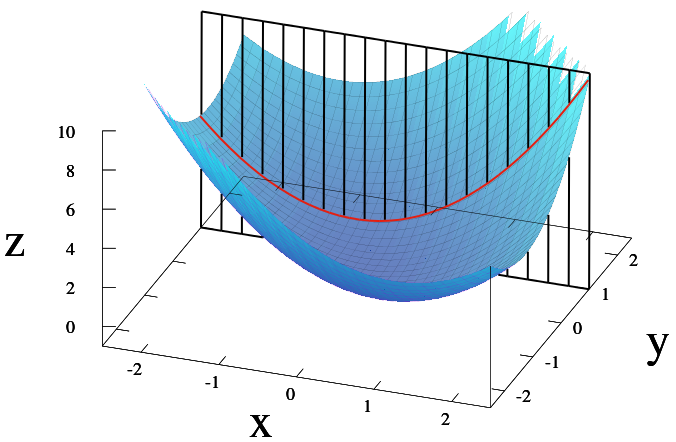
\includegraphics[width=4in]{1.png}

\footnotesize{by \href{https://commons.wikimedia.org/wiki/File:Partial_func_eg.svg}{IkamusumeFan}, CC-BY-SA 4.0}
\end{center}
And we can also generalize this to more vectors, like we turned convex combinations from two vectors to three vectors, and the proof is similar to how we reduced convex combinations from three to two. The general statement is then Jensen's inequality, where for a convex combination $a_1\vec{x_1} + a_2\vec{x_2} + \cdots + a_n\vec{x_n}$, we get
\[
  a_1f(\vec{x_1}) + a_2f(\vec{x_2}) + \cdots + a_nf(\vec{x_n}) \ge f\left(a_1\vec{x_1} + a_2\vec{x_2} + \cdots + a_n\vec{x_n}\right).
\]

\end{document}
